% ------------------------------------------------------------------------------
% TYPO3 CMS 8.1 - What's New (English Version)
%
% @author	Patrick Lobacher <patrick@lobacher.de> and Michael Schams <schams.net>
% @license	Creative Commons BY-NC-SA 3.0
% @link		http://typo3.org/download/release-notes/whats-new/
% @language	English
% ------------------------------------------------------------------------------
% LTXE-CHAPTER-UID:		dcfe6009-2200ad81-816c2edb-1f54c687
% LTXE-CHAPTER-NAME:	Backend User Interface
% ------------------------------------------------------------------------------

\section{Backend User Interface}
\begin{frame}[fragile]
	\frametitle{Backend User Interface}

	\begin{center}\huge{Kapitel 1:}\end{center}
	\begin{center}\huge{\color{typo3darkgrey}\textbf{Backend User Interface}}\end{center}

\end{frame}

% ------------------------------------------------------------------------------
% LTXE-SLIDE-START
% LTXE-SLIDE-UID:		9cbc0864-2e8af1ff-cd11256d-92da1c10
% LTXE-SLIDE-ORIGIN:	5d3d70fa-92a2935e-f1cbdc1e-285ec842 English
% LTXE-SLIDE-TITLE:		Feature: #75497 - inline backend layout wizard
% LTXE-SLIDE-REFERENCE:	!Feature-75497-InlineBackendLayoutWizard.rst
% ------------------------------------------------------------------------------
\begin{frame}[fragile]
	\frametitle{Backend User Interface}
	\framesubtitle{Inline Backend Layout Wizard}

	Es wurde ein neuer Render-Type im TCA zugefügt, um den Backend Layout Wizard der FormEne inline zu rendern
	(im TCA: \texttt{'renderType' => 'belayoutwizard'}).

	\begin{figure}
		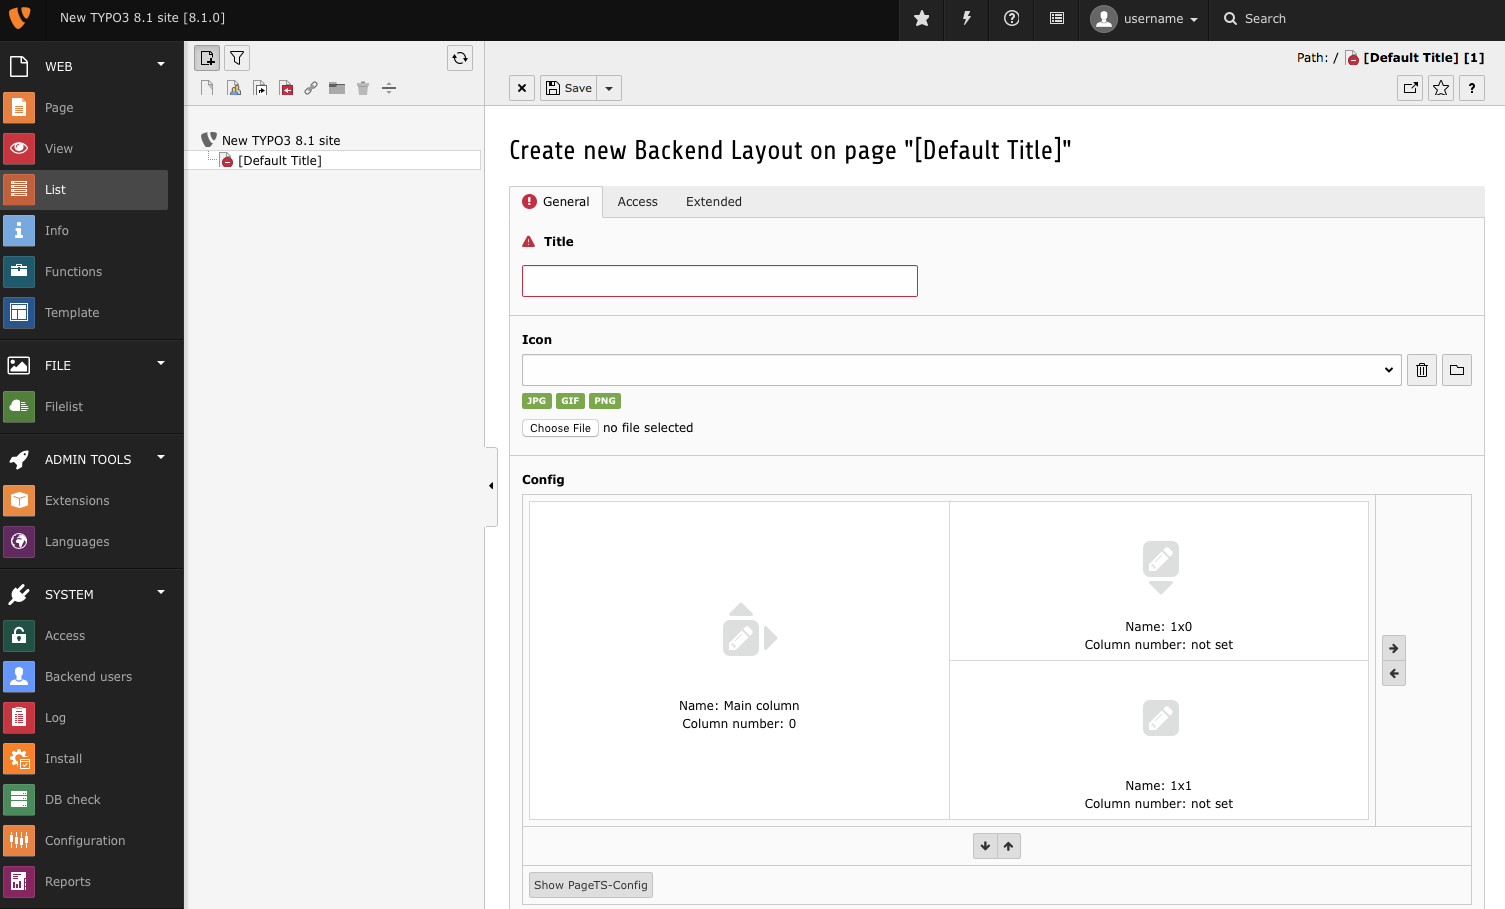
\includegraphics[width=0.70\linewidth]{BackendUserInterface/75497.png}
	\end{figure}

\end{frame}


% ------------------------------------------------------------------------------
% LTXE-SLIDE-START
% LTXE-SLIDE-UID:		05e32ccf-f056b1ed-b6838f97-f8d47ce4
% LTXE-SLIDE-ORIGIN:	7cab4dc0-cdfe9472-a3f0a874-dddf137d English
% LTXE-SLIDE-TITLE:		Feature: #75581 - Simplify cache clearing
% LTXE-SLIDE-REFERENCE:	!Feature-75581-SimplifyCacheClearing.rst
% ------------------------------------------------------------------------------
\begin{frame}[fragile]
	\frametitle{Backend User Interface}
	\framesubtitle{Einfacheres Cache Löschen}

	Das Löschen des Caches wurde vereinfacht, indem Option im Clear Cache Menü und im Install Tool entfernt wurden.

	\begin{itemize}

		\item \textbf{Flush frontend caches:}\newline
			\small
				Löscht die Frontend- und Seiten-bezogenen Caches wie bisher.
			\normalsize

		\item \textbf{Flush all caches:}\newline
			\small
				Löscht alle System-relevanten Caches, wie den Class Loader, Localization, Extension Configuration File-Caches und Opcode Caches. Diesen Cache erneut aufzubauen braucht etwas Zeit.
			\normalsize

	\end{itemize}

	\begin{figure}
		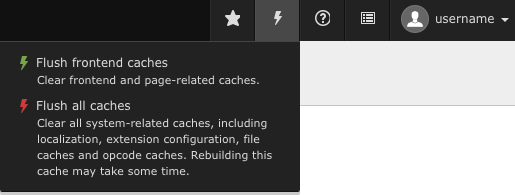
\includegraphics[width=0.45\linewidth]{BackendUserInterface/75581.png}
	\end{figure}

\end{frame}

% ------------------------------------------------------------------------------
% LTXE-SLIDE-START
% LTXE-SLIDE-UID:		2860e7d7-b9956ac8-e2a177f6-44594970
% LTXE-SLIDE-ORIGIN:	e24e593c-fe9bcff9-c386db3a-79491de1 English
% LTXE-SLIDE-TITLE:		Rework Workspaces (1)
% LTXE-SLIDE-REFERENCE:	Rework Workspaces
% ------------------------------------------------------------------------------
\begin{frame}[fragile]
	\frametitle{Backend User Interface}
	\framesubtitle{Überarbeitete Workspaces (1)}

	\begin{itemize}

		\item Das Workspace-Module wurde neu geschrieben und fügt sich viel besser visuell ins Backend ein

		\item Für die visuelle Überarbeitung wurde unter anderem  Twitter Bootstrap und jQuery verwendet

		\item Zusätzlich wurde die Performance erhöht und der Code aufgeräumt, sowie von JavaScript-Balast befreit

	\end{itemize}

\end{frame}

% ------------------------------------------------------------------------------
% LTXE-SLIDE-START
% LTXE-SLIDE-UID:		3f8b14e4-5f2d2f3a-c9ecaab7-86ae0ef2
% LTXE-SLIDE-ORIGIN:	fe9bcff9-e24e593c-79491de1-c386db3a English
% LTXE-SLIDE-TITLE:		Rework Workspaces (2)
% LTXE-SLIDE-REFERENCE:	Rework Workspaces
% ------------------------------------------------------------------------------
\begin{frame}[fragile]
	\frametitle{Backend User Interface}
	\framesubtitle{Überarbeitete Workspaces (2)}

	Screenshots des Workspace-Modules:

	\begin{figure}
		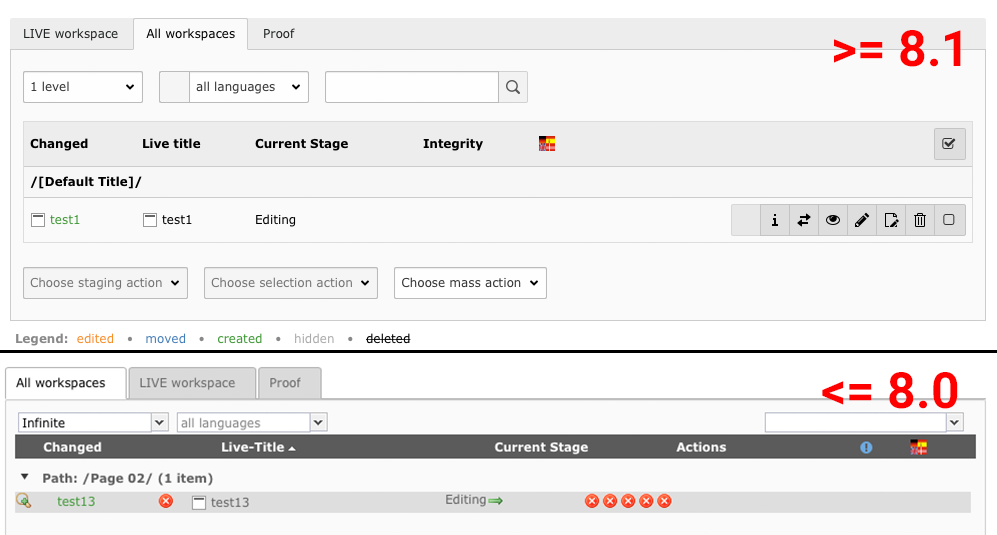
\includegraphics[width=0.85\linewidth]{BackendUserInterface/workspaces.png}
	\end{figure}

\end{frame}

% ------------------------------------------------------------------------------
